\documentclass{article}

\usepackage[margin=1in]{geometry}
\usepackage[backend=bibtex]{biblatex}
\usepackage{graphicx}
\usepackage[english]{babel}

\title{Software Lab Project Report}
\author{Swarupananda (22M2102) and Akshat (190110004)}

\begin{document}

\maketitle

\section{Description of the game}
The name of the Game is “COVID Combat”. It is a 2D game. There is a battlefield consisting of empty places and obstacles through which the active objects (Player and Enemies) of the game can walk and interact. The Player of the Game has an unlimited supply of bullets using which he can kill the enemies. On the other hand, enemies walk randomly and if the Player comes in contact with some enemy, the game is over. If all the enemies are killed, Player wins the game.

\section{What have we achieved}
We've made the 2D version of the game fully functional. This includes rendering the Battlefield i.e. the grid of obstacles onto the canvas. The Player and enemies have been added and their behaviors are all working as expected. Sound effects for background music and shooting bullets have been added. Collision detection between Player and enemies, bullets and enemies have been implemented and based on the collisions we also update the characters. 

Raycasting for the 3D version of the game contains bug and not working properly. This needs some more work.

Following is a snapshot of the 2d version.

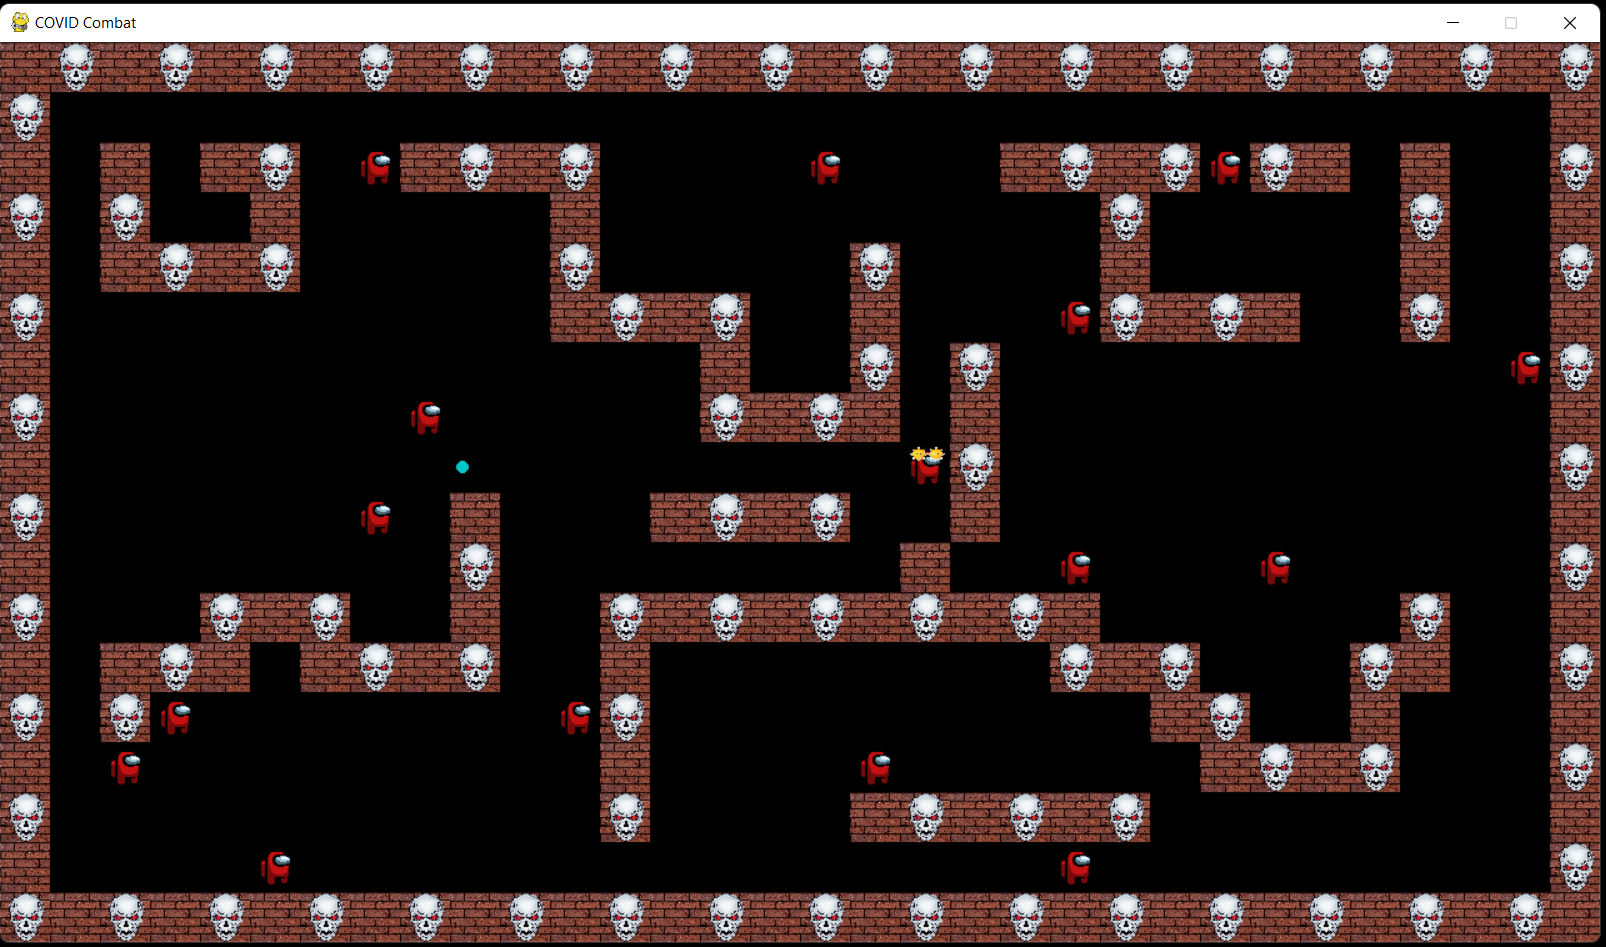
\includegraphics[scale=0.4]{snapshot}

\section{Future Work}
In $Camera.py$ we've some experimental code using which we can cast the 2D grid as a 3D scene and convert this game to a pseudo-3D game. We can add other objects such as sky, floor, hills, trees etc. to make the game look better. Also, we can replace the Player and Enemy images by some realistic characters.

\section{High Level Algorithm}

We first initialize the $enemies$ array with certain number of active enemies. Then in an infinite $while$ loop we do the following things:
\begin{enumerate}
	\item Sleep for sometime
	\item Check if the game is own or over or still running
	\item Process the pygame event queue for user inputs
	\item Update and draw the Player
	\item Draw the grid
	\item Update and draw the alive enemies
	\item Flip the canvas
\end{enumerate}


\section{Documentation}
\textbf{Technologies Used}
\begin{enumerate}
	\item Python and Pygame: For coding the logic of the game
	\item Latex: For creating user manual/documentation for the game
	\item HTML-CSS: A relevant website to give details about the game.
\end{enumerate}

\textbf{Code structure}
\begin{itemize}
	\item main.py
	\begin{enumerate}
		\item This imports the necessary python files and calls the COVID\_Combat.run() method to start the game.
	\end{enumerate}
	\item COVID\_combat.py 
	\begin{enumerate}
		\item Initializes the pygame module
		\item run() : Main game loop. It keeps on checking for user inputs (arrow keys for movements and space key for shooting bullets) and updates the canvas.
	\end{enumerate}
	\item Battlefield.py
	\begin{enumerate}
		\item render\_2d\_grid() : Draws the grid on the canvas in 2D mode
	\end{enumerate}
	\item Player.py
	\begin{enumerate}
		\item update(enemies) : Updates the bullet positions and checks collision between bullet and enemies. Based on collision check, enemies are set to dead if required
		\item change\_position(delta\_position) : Updates player position based on the arrow key clicked. If new position contains an obstacle, position is not updated.
		\item shoot() : Shoots a bullet in the direction in which the Player is currently standing.
		\item rotate\_viewpoint() : Rotates the field of vision of the Player based on mouse events. This will be used in the 3D version of the game.
	\end{enumerate}
	\item Enemy.py
	\begin{enumerate}
		\item update() : Updates position based on random movement. Also checks wall collisions.
	\end{enumerate}
	\item Camera.py
	\begin{enumerate}
		\item take\_snapshot() : The camera at the player's position casts rays to the objects in front of the player within field of vision and projects them onto the screen in 3D mode.
	\end{enumerate}
\end{itemize}

\section{Running Instructions}
To run this game, you need $python3$ and $pygame$. Installation instructions for $python3$ can be found in $www.python.org$ and for $pygame$ in $www.pygame.org$. Once installed, the game can be run by invoking $python main.py$ from the root directory. Use $up, down, left, right$ keys for movements and $space$ key for shooting a bullet. 

\end{document}